\documentclass[11pt]{article}

\usepackage{amsmath,amssymb}
\usepackage{booktabs}
\usepackage{geometry}
\usepackage{graphicx}
\usepackage{hyperref}
\usepackage[numbers,sort&compress]{natbib}

\geometry{margin=1in}
\graphicspath{{plots/}{../plots/}{./}}
\hypersetup{colorlinks=true,linkcolor=blue,citecolor=blue,urlcolor=blue}

\title{Lyman-$\alpha$ forest $P_{1\mathrm{D}}$\\[0.35em]
\large Part I. Linear matter spectrum, Kaiser projection,\\
and optical-depth sightlines}
\author{Helena}
\date{1 November 2026}

\begin{document}
\maketitle

\begin{abstract}
This part specifies the one-dimensional Lyman-$\alpha$ flux power used as the forward model before the discussion of 13~October 2026.
The inputs are the scalar index $n_s$, the primordial amplitude $A_s$, and the linear cold-dark-matter spectrum $P_\mathrm{CDM}$.
The output is $P_{1\mathrm{D}}(k_\parallel,z)$, with $k_\parallel$ in $\mathrm{s\,km}^{-1}$ and $P_{1\mathrm{D}}$ in $\mathrm{km\,s}^{-1}$.
$P_\mathrm{CDM}$ is obtained from the Eisenstein--Hu transfer function, from an external linear table, or from a smooth four-parameter deformation of the Eisenstein--Hu spectrum.
The flux spectrum is then formed in two ways.
The first applies a Kaiser factor at fixed flux bias and integrates out the transverse modes.
The second draws an ensemble of periodic sightlines from the isotropic matter spectrum, maps them to a lognormal density, and assigns a fluctuating Gunn--Peterson optical depth whose amplitude is fixed by a prescribed mean transmission.
The equations, the cosmological assumptions, the numerical resolution, and the relation between the two flux spectra are given below.
\end{abstract}

\section{Scope and fiducial cosmology}
\label{sec:scope}

The calculation returns $P_{1\mathrm{D}}(k_\parallel,z)$ at a single redshift.
The cross-power with a discrete tracer, the covariance of the flux power, and the Fisher matrix lie outside this part.
Both flux spectra defined below are built from the same $P_\mathrm{CDM}$, so that a change in the matter spectrum enters each of them in a controlled way.
The Kaiser spectrum is a smooth function of $n_s$ and $A_s$.
The sightline spectrum is a realisation of a random field at fixed cosmological parameters, and is used to test the flux model.

Every numerical illustration in this part uses the same fiducial point,
\begin{equation}
\label{eq:fiducial}
\begin{aligned}
\Omega_m &= 0.31, &
\Omega_b &= 0.049, &
h &= 0.67, \\
n_s &= 0.965, &
A_s &= 2.1\times 10^{-9}, &
z &= 3.
\end{aligned}
\end{equation}
The background is a flat $\Lambda$CDM cosmology with massless neutrinos.
The density parameters and $h$ are a rounded Planck-like choice, held fixed so that variations of $n_s$, $A_s$, and redshift can be read separately.
The Hubble parameter is
\begin{equation}
\label{eq:hubble}
H(z) = 100\,h \sqrt{\Omega_m(1+z)^{3} + 1 - \Omega_m},
\end{equation}
in $\mathrm{km\,s}^{-1}\,\mathrm{Mpc}^{-1}$.
Comoving separations are converted to the velocity units of a forest spectrum by
\begin{equation}
\label{eq:units}
\frac{\mathrm{d}v}{\mathrm{d}\chi}
=
\frac{H(z)}{(1+z)\,h},
\end{equation}
in $\mathrm{km\,s}^{-1}$ per comoving $\mathrm{Mpc}/h$.
A wavenumber transforms as $k\,[h\,\mathrm{Mpc}^{-1}] = k\,[\mathrm{s\,km}^{-1}]\,\mathrm{d}v/\mathrm{d}\chi$, and a one-dimensional power transforms as $P_{1\mathrm{D}}\,[\mathrm{km\,s}^{-1}] = P_{1\mathrm{D}}\,[\mathrm{Mpc}/h]\,\mathrm{d}v/\mathrm{d}\chi$.
At the fiducial redshift this factor equals $113\,\mathrm{km\,s}^{-1}$ per $\mathrm{Mpc}/h$.
The interval $10^{-3}$--$0.02\,\mathrm{s\,km}^{-1}$, which is the range shown for the forest power, therefore corresponds to $0.11$--$2.3\,h\,\mathrm{Mpc}^{-1}$, or to comoving wavelengths from about $55\,\mathrm{Mpc}/h$ down to about $3\,\mathrm{Mpc}/h$.

\section{Linear matter power spectrum}
\label{sec:matter}

\subsection{Eisenstein--Hu spectrum}
\label{sec:eh}

The default three-dimensional spectrum is the Eisenstein and Hu fitting formula for the matter transfer function in a baryon--cold-dark-matter universe \citep{Eisenstein:1997ik}.
Inside the transfer function the wavenumber is in $\mathrm{Mpc}^{-1}$.
The fit is normalised to $T(k\to 0)=1$ and retains the baryon acoustic oscillations.
Because the expression is closed, $n_s$ and $A_s$ can be varied without a further Boltzmann solution.
On a comparison with CAMB at $z=0$, over $10^{-3}$--$10\,h\,\mathrm{Mpc}^{-1}$, the median ratio of the two spectra is approximately $1.01$.

The linear power in $\mathrm{Mpc}^{3}$ is
\begin{equation}
\label{eq:pcdm}
P(k,z)
=
\frac{8\pi^{2}}{25}
\frac{A_s}{\Omega_m^{2} H_0^{4}}
\left(\frac{k}{k_\mathrm{pivot}}\right)^{n_s-1}
k\,T(k)^{2}\,D(z)^{2},
\end{equation}
with primordial pivot $k_\mathrm{pivot}=0.05\,\mathrm{Mpc}^{-1}$ and $H_0 = 100h/299792.458$ in $\mathrm{Mpc}^{-1}$.
Multiplication by $h^{3}$ converts $P$ to $(\mathrm{Mpc}/h)^{3}$.
The linear growth factor for the flat background \eqref{eq:hubble} is
\begin{equation}
\label{eq:growth}
D(a)
=
\frac{5}{2}\,\Omega_m\,E(a)
\int_{0}^{a}
\frac{\mathrm{d}a'}{\bigl[a' E(a')\bigr]^{3}},
\qquad
E(a)=\frac{H(a)}{H_0},
\end{equation}
with $a=1/(1+z)$.
This normalisation enforces $D(a)\to a$ during matter domination.
The integral is evaluated numerically from deep in the matter era.

\subsection{External linear table}
\label{sec:table}

Equation~\eqref{eq:pcdm} may be replaced by a two-column table.
The first column is $k$ in $h\,\mathrm{Mpc}^{-1}$.
The second is the linear $P(k)$ in $(\mathrm{Mpc}/h)^{3}$ at one fiducial redshift, already containing the fiducial $n_s$ and $A_s$.
The table is interpolated with a monotone piecewise-cubic interpolant in $\ln k$ and $\ln P$.
Evaluation is restricted to the interval covered by the file.
A subsequent change of amplitude, tilt, or redshift rescales the stored spectrum,
\begin{equation}
\label{eq:table}
P(k)
=
P_\mathrm{fid}(k)\,
\frac{A_s}{A_{s,\mathrm{fid}}}\,
\left(\frac{k}{k_p}\right)^{n_s-n_{s,\mathrm{fid}}}\,
\left(\frac{D(z)}{D(z_\mathrm{fid})}\right)^{2},
\end{equation}
with pivot $k_p = 0.05/h$ in $h\,\mathrm{Mpc}^{-1}$.
If the requested redshift is the redshift of the file, the growth ratio is unity.
A CLASS spectrum written in $\mathrm{Mpc}^{-1}$ and $\mathrm{Mpc}^{3}$ is converted by $k_h=k/h$ and $P_h = P\,h^{3}$ before it is read.
A CAMB matter-power file is already in these $h$ units.
The table is required to be the linear spectrum.
Once it has been supplied, $n_s$, $A_s$, and $\Omega_b$ determine only the rescaling \eqref{eq:table}.
The redshift, $\Omega_m$, and $h$ still enter the unit conversion \eqref{eq:units}.
For the Kaiser projection of Sec.~\ref{sec:kaiser} the table must extend through the numerical cutoff $30\,h\,\mathrm{Mpc}^{-1}$.

\subsection{Four-parameter deformation}
\label{sec:abgd}

A smooth deformation of the Eisenstein--Hu spectrum is available for shape variations about the fiducial model,
\begin{equation}
\label{eq:abgd}
P(k)
=
P_\mathrm{EH}(k)\,
\exp\bigl(\alpha L + \beta L^{2} + \gamma L^{3} + \delta L^{4}\bigr),
\qquad
L = \ln(k/k_p),
\end{equation}
with $k_p = 1\,h\,\mathrm{Mpc}^{-1}$.
At the pivot, $L=0$ and the exponential equals one, so the amplitude remains that of Eq.~\eqref{eq:pcdm}.
Vanishing coefficients recover the Eisenstein--Hu spectrum exactly.
The symbol $\gamma$ in Eq.~\eqref{eq:abgd} is a coefficient of the matter spectrum.
It is distinct from the temperature--density index of Sec.~\ref{sec:fgpa}.

\section{Analytic flux power}
\label{sec:kaiser}

\subsection{Redshift-space model}

On scales where the forest may be treated as a linearly biased tracer in coherent infall, the three-dimensional flux power is the Kaiser form \citep{Kaiser:1987qv,McDonald:2001fe}
\begin{equation}
\label{eq:kaiser}
P_F(k,\mu)
=
b_F^{2}\,(1+\beta_F\mu^{2})^{2}\,P_\mathrm{CDM}(k),
\qquad
\mu = k_\parallel/k.
\end{equation}
The fiducial parameters are
\begin{equation}
\label{eq:bias}
b_F = -0.14, \qquad \beta_F = 1.4,
\end{equation}
held fixed at every redshift.
The sign of $b_F$ follows from the physics of the forest: an overdensity raises the neutral fraction, raises the optical depth, and lowers the transmission.
In the original galaxy derivation, $\beta_F$ is the ratio of the logarithmic growth rate to the tracer bias \citep{Kaiser:1987qv}.
Here $\beta_F$ is specified directly, as is standard in forest analyses, and is independent of the optical-depth exponent introduced in Sec.~\ref{sec:fgpa}.

The pair \eqref{eq:bias} is a round representation of the large-scale Lyman-$\alpha$ bias measured in early DESI data,
$b_{\mathrm{Ly}\alpha} = -0.134 \pm 0.009$ and $\beta_{\mathrm{Ly}\alpha} = 1.41^{+0.12}_{-0.15}$ \citep{Gordon:2023dua}.
The eBOSS and DESI analyses also multiply the bias by a redshift factor $(1+z)^{2.9}$ about a pivot redshift \citep{eBOSS:2020tmo}.
That factor is omitted here: $b_F$ and $\beta_F$ take the values \eqref{eq:bias} at every $z$ used in the calculation.
McDonald's additional scale-dependent factors, which describe nonlinear growth, gas pressure, and nonlinear velocities, are likewise omitted from Eq.~\eqref{eq:kaiser} \citep{McDonald:2001fe}.

\subsection{Line-of-sight projection}

A forest spectrum measures only the line-of-sight wavenumber.
Under the Fourier convention in which the three-dimensional variance is $\int \mathrm{d}^{3}k\,P_F(k)/(2\pi)^{3}$, the perpendicular plane integrates to
\begin{equation}
\label{eq:p1d}
P_{1\mathrm{D}}(k_\parallel)
=
\int_{k_\parallel}^{k_\mathrm{max}}
\frac{k\,\mathrm{d}k}{2\pi}\,
P_F\!\left(k,\,\mu=\frac{k_\parallel}{k}\right).
\end{equation}
The lower limit follows because a three-dimensional mode of wavenumber $k$ has line-of-sight component $k_\parallel = \mu k$ with $|\mu|\le 1$, and therefore contributes only to $k_\parallel \le k$.
The integral is evaluated by the trapezoidal rule on $800$ logarithmically spaced samples.
The upper limit is the numerical cutoff
\begin{equation}
k_\mathrm{max} = 30\,h\,\mathrm{Mpc}^{-1}.
\end{equation}
It lies above the forest window of Sec.~\ref{sec:scope}.
Power at high $k$ still contributes to $P_{1\mathrm{D}}$ at a lower $k_\parallel$, so the cutoff must be carried past the scales at which the spectrum is plotted.
It is a property of the quadrature.
Gas pressure is expected to remove power near $10$--$20\,h\,\mathrm{Mpc}^{-1}$ \citep{McDonald:2001fe}, and Eq.~\eqref{eq:p1d} retains that power because Eq.~\eqref{eq:kaiser} contains no pressure term.

\subsection{Regime of validity}

Equation~\eqref{eq:kaiser} assumes a density contrast small enough for a constant bias, together with coherent peculiar velocities.
It ceases to describe the forest where the map $F=e^{-\tau}$ is nonlinear, where saturated lines no longer respond to a further increase in density, where randomised motions suppress the $\mu\sim 1$ modes, or where a single $b_F$ cannot represent strong overdensities and gas affected by galactic feedback \citep{Kooistra:2022hzw}.
Those scales are still inside the integral \eqref{eq:p1d}.
The analytic $P_{1\mathrm{D}}$ at forest wavenumbers therefore includes a small-scale contribution computed outside the regime in which the Kaiser factor was derived.

\section{Optical-depth sightlines}
\label{sec:sightlines}

The second flux spectrum is measured on periodic lines of sight drawn from $P_\mathrm{CDM}$.
The lines are constructed in one dimension.
For a statistically isotropic Gaussian field, the power along any one line is fixed by $P_\mathrm{CDM}$ before a three-dimensional volume is generated, and that reduced description is what the estimator below requires.

\subsection{Isotropic projection}
\label{sec:projection}

With the same Fourier convention as in Eq.~\eqref{eq:p1d}, isotropy reduces the transverse integral to
\begin{equation}
\label{eq:matter1d}
P_{1\mathrm{D},\mathrm{matter}}(k_\parallel)
=
\frac{1}{2\pi}
\int_{k_\parallel}^{q_\mathrm{max}}
q\,P_\mathrm{CDM}(q)\,\mathrm{d}q.
\end{equation}
The integrand is the matter spectrum $P_\mathrm{CDM}(q)$.
The upper limit is the last wavenumber stored in the matter table.
The integral is a cumulative trapezoidal rule taken from that upper limit, then interpolated onto the Fourier modes of the line.
The quadrature uses $8192$ logarithmically spaced samples across the table.

\subsection{Gaussian realisation}
\label{sec:gaussian}

A line of comoving length $L$ is divided into $N$ pixels of size $\mathrm{d}x=L/N$.
Its Fourier modes are $k_j = 2\pi j/L$, from the fundamental mode $2\pi/L$ to the Nyquist mode $\pi N/L$ when $N$ is even.
The matter table must cover this entire set of modes.
Each line is drawn so that its discrete one-dimensional spectrum equals Eq.~\eqref{eq:matter1d}.
In the normalisation where the field is recovered by an unnormalised inverse real transform, the complex coefficient at $0<k<k_\mathrm{Nyquist}$ has variance $N^{2} P_{1\mathrm{D},\mathrm{matter}}(k)/L$, split equally between the real and imaginary parts.
The Nyquist coefficient, when $N$ is even, is real and carries the full variance $N^{2} P_{1\mathrm{D},\mathrm{matter}}/L$.
The zero mode is set identically to zero, so each line has vanishing mean contrast.
Distinct lines are independent draws.
A single line has the same one-dimensional power as a row through an isotropic Gaussian volume.
Transverse correlations are a property of the volume, so $P_F(k,\mu)$ and a cross-power require a three-dimensional realisation.

The comparison figure of Sec.~\ref{sec:figures} uses $L=200\,\mathrm{Mpc}/h$, $N=512$, and $256$ lines.
The pixel is then $0.391\,\mathrm{Mpc}/h$, about $44\,\mathrm{km\,s}^{-1}$ at $z=3$, and the Nyquist wavenumber is $\pi N/L \approx 8.0\,h\,\mathrm{Mpc}^{-1}$, about $0.07\,\mathrm{s\,km}^{-1}$.
The default configuration of the implementation is the same length and the same number of lines, with $N=1024$.

\subsection{Lognormal density and optical depth}
\label{sec:fgpa}

The Gaussian contrast $\delta_G$ is mapped to a positive density contrast by the lognormal transformation \citep{Coles:1991if,Bi:1996fh},
\begin{equation}
\label{eq:lognormal}
\Delta
=
\exp\!\left(\delta_G - \tfrac12 \mathrm{Var}(\delta_G)\right).
\end{equation}
The subtraction of half the variance sets the spatial mean of $\Delta$ close to unity.
In photoionisation equilibrium the neutral hydrogen density scales as $n_\mathrm{H}^{2}\,\alpha_B(T)/\Gamma$.
With $n_\mathrm{H}\propto\Delta$, $T=T_0\Delta^{\gamma-1}$, and a recombination coefficient $\alpha_B\propto T^{-0.7}$, the Gunn--Peterson optical depth scales as a power of the density \citep{Gunn:1965hd,Hui:1997dp},
\begin{equation}
\label{eq:fgpa}
\beta = 2 - 0.7\,(\gamma - 1),
\qquad
\tau = A\,\Delta^{\beta},
\qquad
F = e^{-\tau}.
\end{equation}
The fiducial temperature--density index is $\gamma=1.5$, which gives $\beta=1.65$.
This exponent $\beta$ is a property of the recombination rate.
It is a different quantity from the redshift-space parameter $\beta_F$ in Eq.~\eqref{eq:kaiser}.

The amplitude $A$ is the remaining degree of freedom in $\tau$.
It is determined by requiring the mean transmission, averaged over every pixel of every line, to equal a specified target.
The root is taken in $\ln A$.
The target used throughout this part is $\langle F\rangle = 0.80$.
For the $256$ lines of the comparison figure the solution is $A=0.485$.
The target is an input of the model.
At $z=3$ the observed mean transmission of the forest lies closer to $0.7$.

For a small contrast $\Delta=1+\delta$ with vanishing mean, the transmission linearises to $\delta_F \approx -A\beta\,\delta$.
On the comparison lines, $A\beta \approx 0.80$.
The linear response implied by Eqs.~\eqref{eq:lognormal}--\eqref{eq:fgpa} is therefore several times larger than the large-scale bias $b_F=-0.14$ adopted in Eq.~\eqref{eq:bias}.
The two calculations are normalised by different conditions: a measured large-scale bias in one case, and a mean transmission in the other.

Pressure smoothing and thermal broadening are implemented as periodic Gaussian convolutions along the line, in pixel units.
Both widths are set to zero in every result of this part.
A line-of-sight displacement may be supplied externally, in which case $\tau$ is shifted by cloud-in-cell interpolation before the thermal convolution.
The spectra shown here are real-space spectra: no displacement is applied.
Arya et al.\ combine the same lognormal density and $\tau\propto\Delta^{\beta}$ sequence with a Jeans cutoff, and they determine $A$ from the temperature and the photoionisation rate \citep{Arya:2022uke}.
In this part $A$ is fixed by $\langle F\rangle$, and the lines are left unsmoothed.

\subsection{Flux-power estimator}
\label{sec:estimator}

The flux contrast on each line is
\begin{equation}
\label{eq:deltaf}
\delta_F = \frac{F}{\langle F\rangle} - 1,
\end{equation}
where the average runs over the whole ensemble.
Its one-dimensional power is the ensemble mean of the periodogram.
With $\tilde\delta_F$ the unnormalised discrete Fourier coefficient,
\begin{equation}
\label{eq:periodogram}
P_{1\mathrm{D}}(k)
=
\frac{(\mathrm{d}x)^{2}}{L}
\left\langle \bigl|\tilde\delta_F(k)\bigr|^{2} \right\rangle.
\end{equation}
Equation~\eqref{eq:units} converts this comoving spectrum to $\mathrm{km\,s}^{-1}$.
The variance assigned in Sec.~\ref{sec:gaussian} is the inverse of this normalisation, so a Gaussian line drawn from Eq.~\eqref{eq:matter1d} returns that spectrum under Eq.~\eqref{eq:periodogram}.

\subsection{Further limitations of the sightline model}

On the comparison lines, with pressure smoothing omitted, the variance of the lognormal density is approximately $19$.
The field is therefore far outside the small-contrast expansion used to relate $A\beta$ to $b_F$.
Kooistra, Lee, and Horowitz show that $\tau\propto\Delta^{\beta}$ itself fails in strong overdensities and in gas affected by galactic feedback \citep{Kooistra:2022hzw}.
Arya, Paranjape, and Choudhury find that, in their lognormal model, dropping the longest modes along a sightline can shift the inferred gas parameters by about $2\sigma$, whereas the covariance between neighbouring $k$ bins has a weaker effect on the inference \citep{Arya:2023ipe}.
The lines used here have length $200\,\mathrm{Mpc}/h$, fundamental mode $2\pi/L$, and a mean mode set to zero.
A subsequent paper of that series reports that a plain lognormal density does not reproduce the flux probability distribution and its redshift evolution from $z=2$ to $z=2.7$, and introduces one extra parameter in the width of the distribution \citep{Arya:2023fal}.
The sightlines of this part use Eq.~\eqref{eq:lognormal} with the variance measured on the ensemble.

\section{Relation between the two flux spectra}
\label{sec:relation}

The two spectra are both called $P_{1\mathrm{D}}$, and they are evaluated in the same units, but they are different functionals of $P_\mathrm{CDM}$.

The analytic spectrum is Eq.~\eqref{eq:p1d} applied to Eq.~\eqref{eq:kaiser}.
Its amplitude is set by $b_F^{2}$ and by $\mathrm{d}v/\mathrm{d}\chi$.
Redshift-space distortions are present through $\beta_F$.
The density enters linearly, and the small-scale contribution is whatever $P_\mathrm{CDM}$ supplies up to $30\,h\,\mathrm{Mpc}^{-1}$.
A fractional change in $A_s$ rescales this $P_{1\mathrm{D}}$ by the same fraction at every $k_\parallel$.
A change in $n_s$ tilts it.
Parameter derivatives are well defined on this spectrum.

The sightline spectrum is Eq.~\eqref{eq:periodogram} applied to the transmission \eqref{eq:fgpa}.
Its amplitude is set by the requirement $\langle F\rangle=0.80$.
The lines are real-space lines, the map from density to flux is exponential, and the density variance on the comparison lines is large.
The result depends on the random seed.
Increasing the number of lines reduces the scatter of the measured spectrum as $N_\mathrm{lines}^{-1/2}$.
The offset from the Kaiser curve remains, because the two spectra are normalised and distorted by different operations.

Dividing each spectrum by its own value at $k_\parallel=0.005\,\mathrm{s\,km}^{-1}$ removes the normalisation.
Over the forest window the shapes then agree, which is the content of the last figure in Sec.~\ref{sec:figures}.
Agreement of the amplitudes, in real space and on scales where $\delta$ remains small, would additionally require $b_F=-A\beta$ and $\beta_F=0$, together with the same small-scale suppression in both calculations.
The angular factor $(1+\beta_F\mu^{2})^{2}$ arises from peculiar velocities sourced by modes perpendicular to the line of sight, which are defined in a three-dimensional realisation.

\section{Numerical illustrations}
\label{sec:figures}

The eight figures were produced at the fiducial point \eqref{eq:fiducial}, with the deformations and redshift variations stated in the captions.
The sightline panels use $L=200\,\mathrm{Mpc}/h$, $N=512$, $256$ lines, temperature--density index $\gamma=1.5$, target mean transmission $0.80$, and vanishing pressure and thermal widths.
For that ensemble the fitted amplitude is $A=0.485$ and the mean transmission is $0.80$.

\begin{figure}[htbp]
\centering
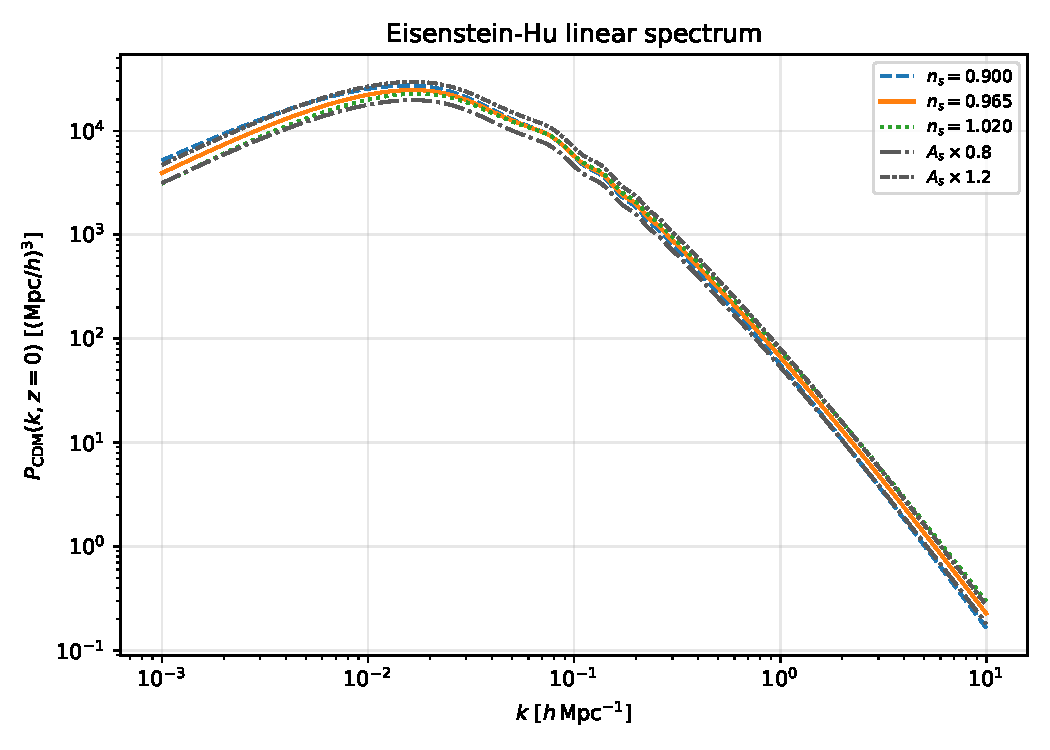
\includegraphics[width=0.92\textwidth]{01_pcdm_ns_As.pdf}
\caption{Linear matter spectrum $P_\mathrm{CDM}(k)$ at $z=0$.
A lower $n_s$ increases the large-scale power relative to the fiducial index.
A change in $A_s$ rescales the spectrum uniformly.}
\label{fig:pcdm}
\end{figure}

\begin{figure}[htbp]
\centering
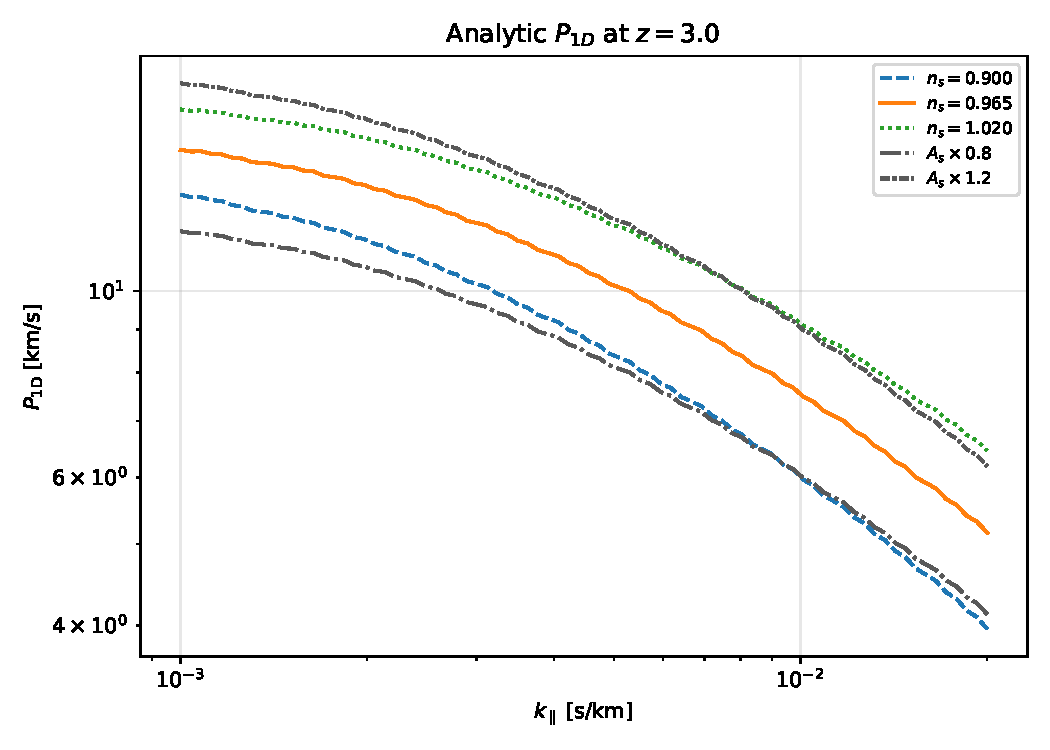
\includegraphics[width=0.92\textwidth]{02_p1d_ns_As.pdf}
\caption{Kaiser one-dimensional flux power at $z=3$, from Eqs.~\eqref{eq:kaiser} and \eqref{eq:p1d}, for the same variations of $n_s$ and $A_s$ as in Fig.~\ref{fig:pcdm}.
Units are $\mathrm{km\,s}^{-1}$.}
\label{fig:p1d-ns-as}
\end{figure}

\begin{figure}[htbp]
\centering
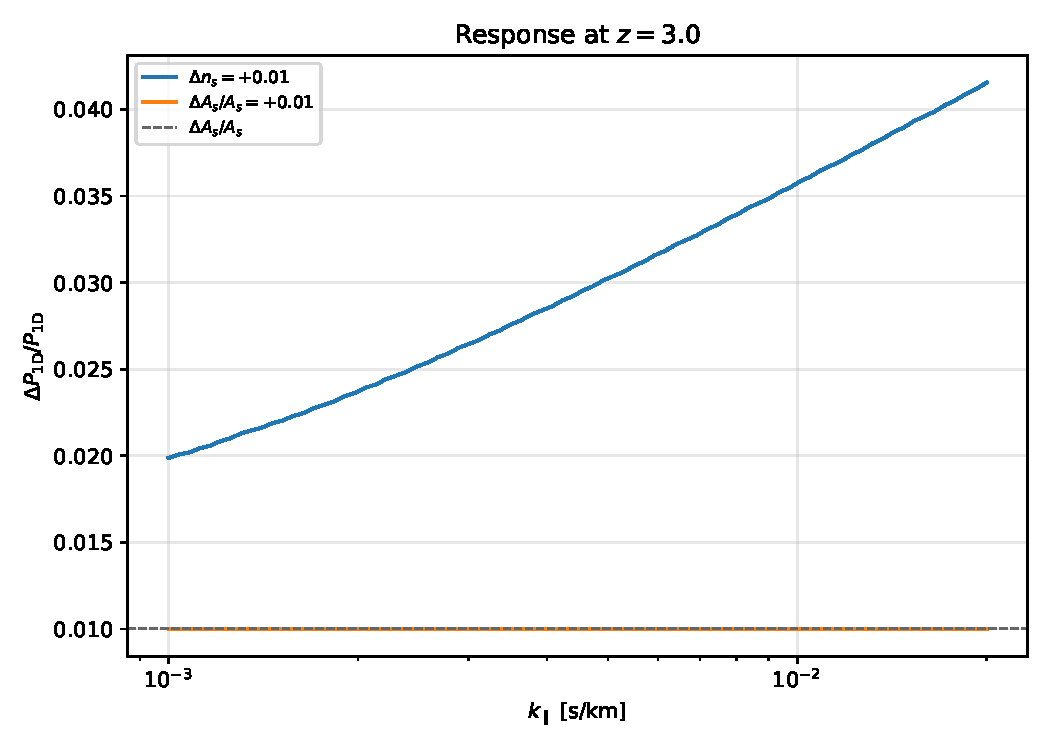
\includegraphics[width=0.92\textwidth]{03_p1d_fractional.pdf}
\caption{Fractional response of the Kaiser $P_{1\mathrm{D}}$ at $z=3$.
A one percent increase in $A_s$ raises $P_{1\mathrm{D}}$ by one percent at every $k_\parallel$.
An increase of $n_s$ by $0.01$ produces a scale-dependent change of about two to four percent across the plotted window.}
\label{fig:p1d-frac}
\end{figure}

\begin{figure}[htbp]
\centering
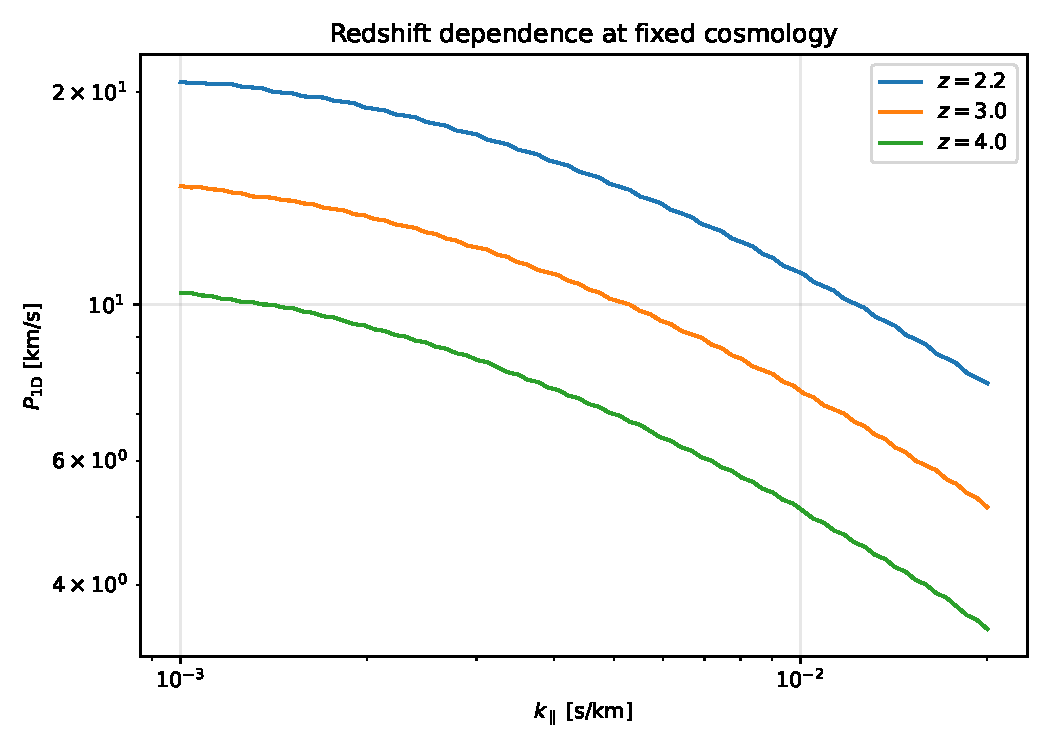
\includegraphics[width=0.92\textwidth]{04_p1d_redshifts.pdf}
\caption{Kaiser $P_{1\mathrm{D}}$ at $z=2.2$, $3$, and $4$, with $b_F$ and $\beta_F$ held at Eq.~\eqref{eq:bias}.
The amplitude changes through the growth function $D(z)$ and through the unit conversion \eqref{eq:units}.}
\label{fig:p1d-z}
\end{figure}

\begin{figure}[htbp]
\centering
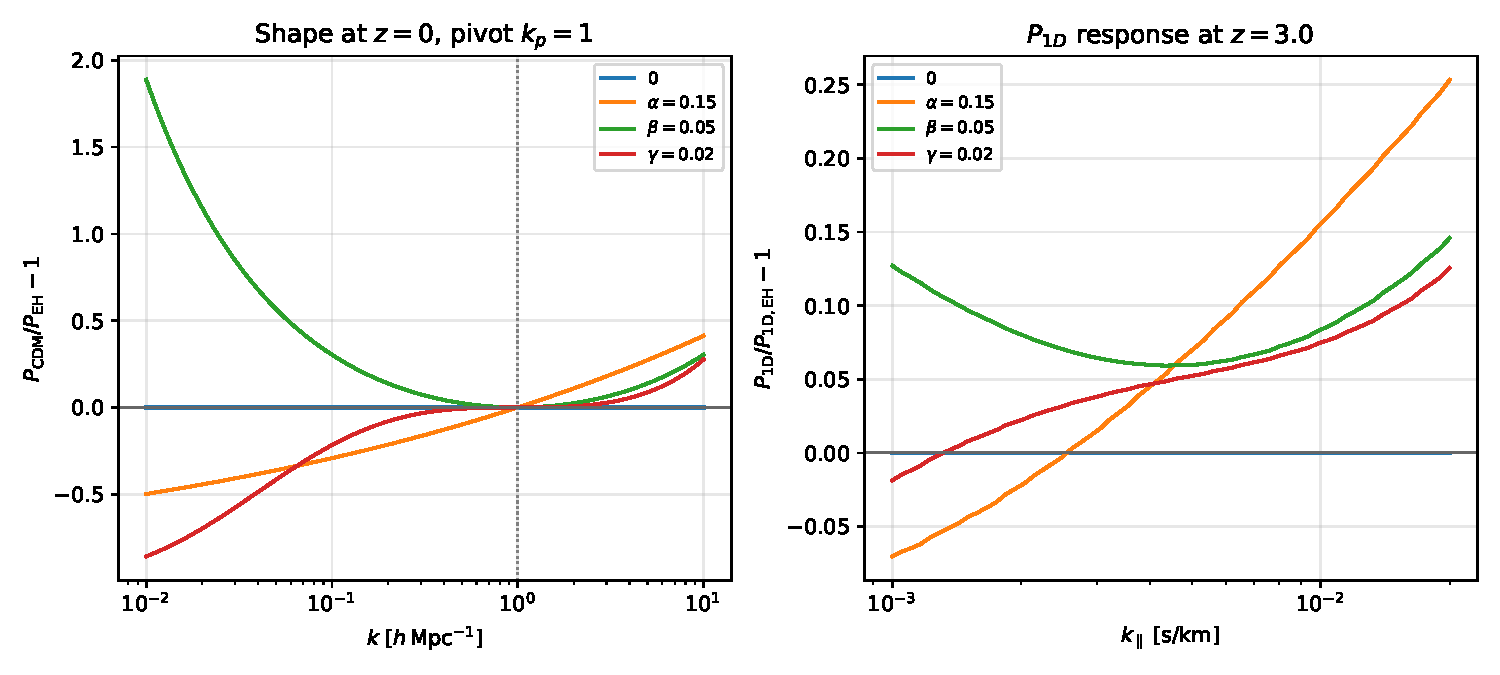
\includegraphics[width=0.92\textwidth]{05_abgd_shape.pdf}
\caption{Four-parameter deformation \eqref{eq:abgd}.
Each of $\alpha$, $\beta$, and $\gamma$ is varied separately about the Eisenstein--Hu spectrum.
On $P_\mathrm{CDM}$ the fractional change vanishes at the pivot $k_p=1\,h\,\mathrm{Mpc}^{-1}$.
Vanishing coefficients recover the Eisenstein--Hu spectrum.}
\label{fig:abgd}
\end{figure}

\begin{figure}[htbp]
\centering
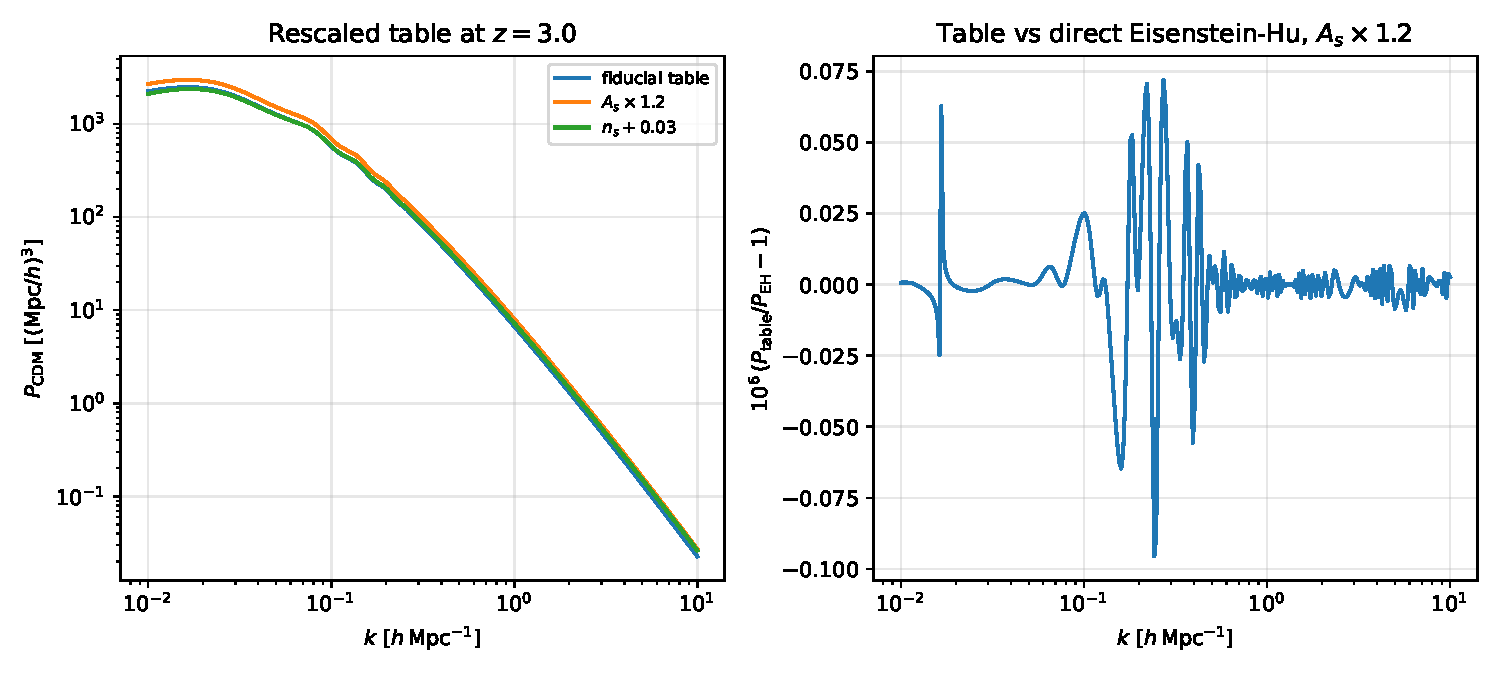
\includegraphics[width=0.92\textwidth]{06_table_rescaling.pdf}
\caption{External matter table after the rescaling \eqref{eq:table} in $A_s$ or $n_s$, compared with a direct evaluation of Eq.~\eqref{eq:pcdm}.
The fractional residual is at the level of $10^{-6}$.}
\label{fig:table}
\end{figure}

\begin{figure}[htbp]
\centering
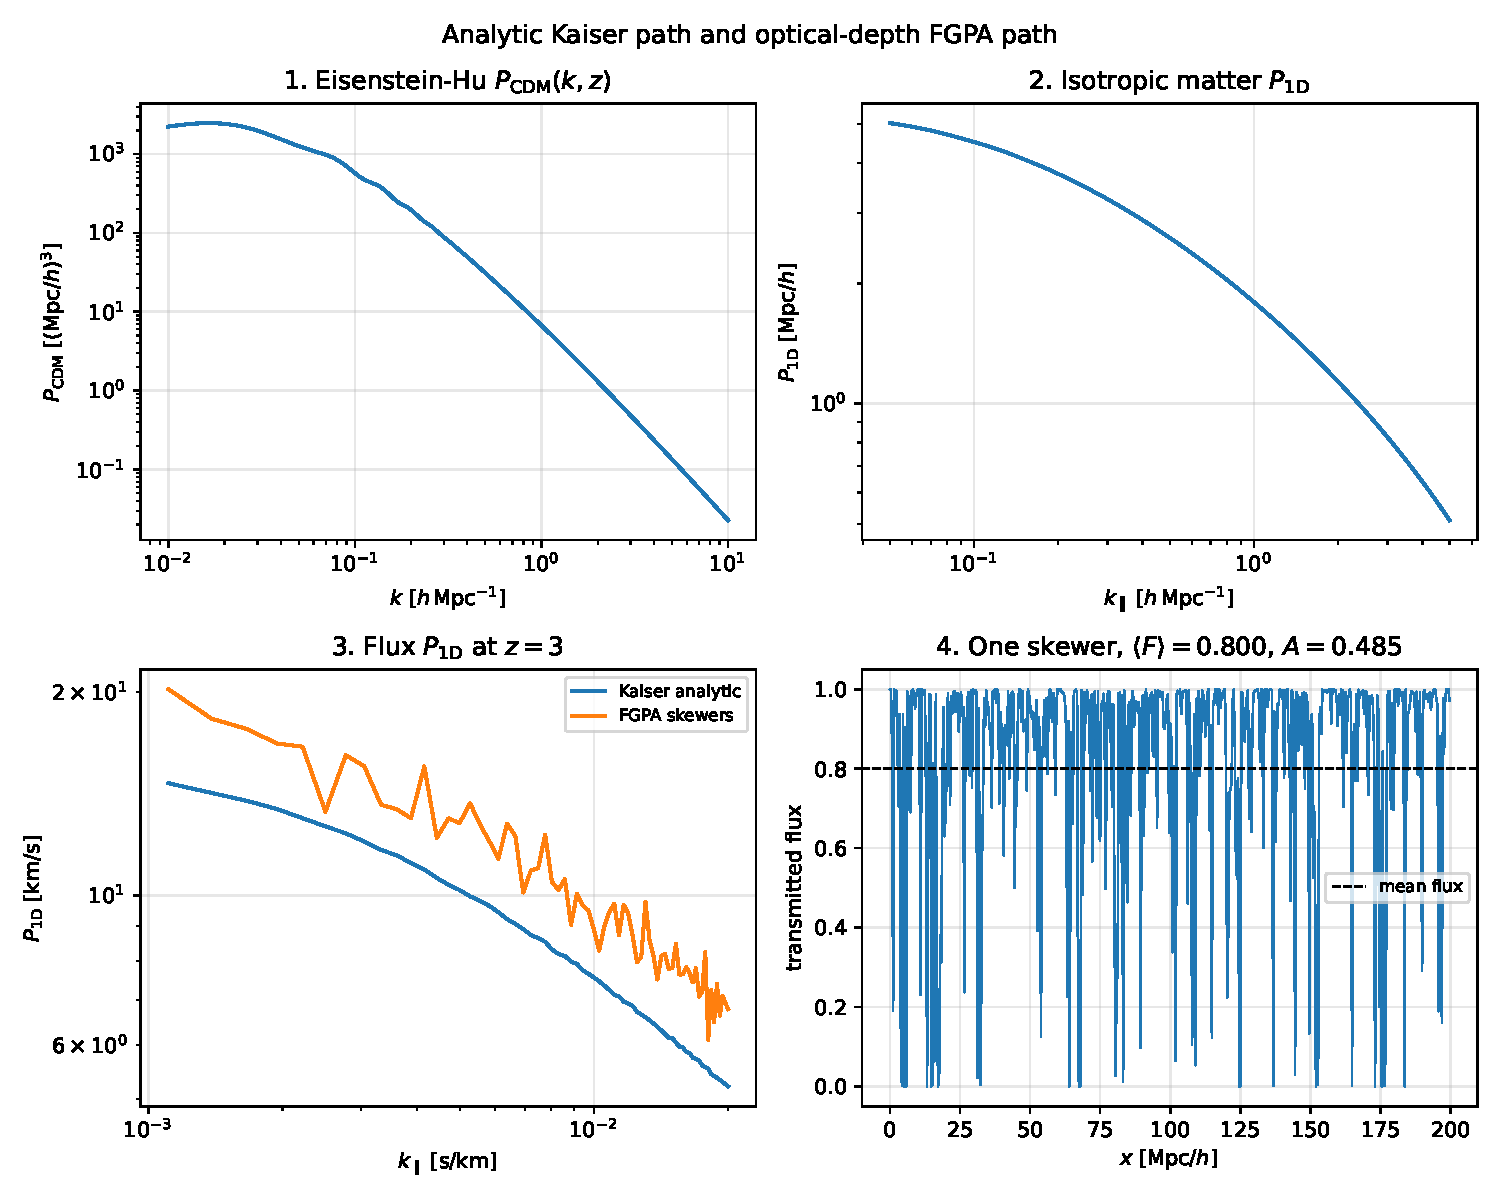
\includegraphics[width=\textwidth]{07_pipeline_stages.pdf}
\caption{Pipeline stages at the fiducial point.
Top left: three-dimensional matter spectrum.
Top right: isotropic line-of-sight projection of that spectrum.
Bottom left: Kaiser flux power and the mean of $256$ optical-depth sightlines, in absolute units.
Bottom right: one transmitted-flux line; for this ensemble $\langle F\rangle=0.80$ and $A=0.485$.}
\label{fig:pipeline}
\end{figure}

\begin{figure}[htbp]
\centering
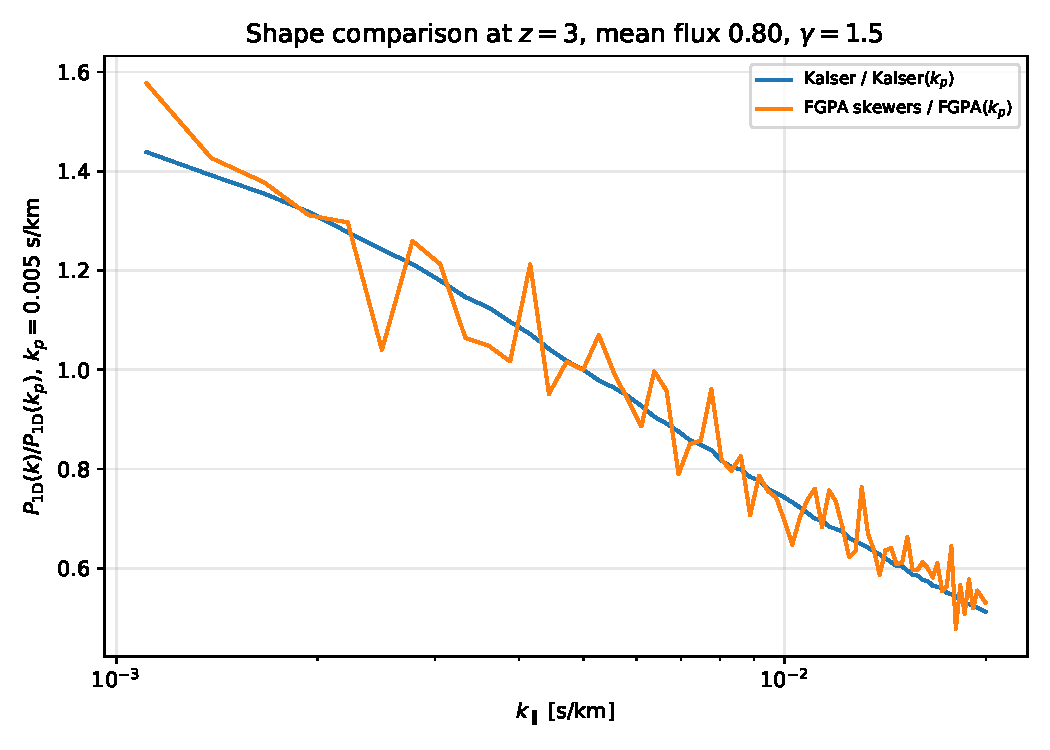
\includegraphics[width=0.88\textwidth]{08_kaiser_vs_fgpa_shape.pdf}
\caption{Same flux spectra as in Fig.~\ref{fig:pipeline}, each divided by its value at $k_\parallel=0.005\,\mathrm{s\,km}^{-1}$.
The shapes agree across the forest window.
The residual variation of the sightline curve is the sampling noise of the finite ensemble.}
\label{fig:shape}
\end{figure}

\appendix
\section{Implementation}
\label{sec:code}

The calculation is the Python package \texttt{p1d} in the repository \texttt{fisher-forecasts-future-spectroscopic-survey}.
The equations of this note are assigned to the following functions.

\begin{center}
\small
\begin{tabular}{@{}p{0.46\textwidth}p{0.48\textwidth}@{}}
\toprule
Operation & Function \\
\midrule
$T(k)$, $D(z)$, and Eq.~\eqref{eq:pcdm} &
\texttt{linear\_matter\_power} in \texttt{eisenstein\_hu.py} \\
Table, interpolation, and Eq.~\eqref{eq:table} &
\texttt{TabulatedMatterPower} in \texttt{matter\_table.py} \\
Equation~\eqref{eq:abgd} &
\texttt{p1d\_skm\_abgd} in \texttt{abgd.py} \\
Equations~\eqref{eq:kaiser} and \eqref{eq:p1d}, and the unit conversion &
\texttt{p1d\_skm} in \texttt{flux.py} \\
Equation~\eqref{eq:matter1d} &
\texttt{project\_p1d} in \texttt{projection.py} \\
Gaussian lines and Eq.~\eqref{eq:periodogram} &
\texttt{generate\_gaussian\_skewers}, \texttt{measure\_p1d} in \texttt{skewers.py} \\
Equations~\eqref{eq:lognormal}--\eqref{eq:deltaf} and the solution for $A$ &
\texttt{run\_fgpa\_skewers} in \texttt{fgpa\_field.py} \\
\bottomrule
\end{tabular}
\end{center}

\noindent
The entry point for the analytic spectrum is \texttt{p1d\_skm}.
Its arguments are $k_\parallel$ in $\mathrm{s\,km}^{-1}$, redshift, $n_s$, $A_s$, $\Omega_m$, $\Omega_b$, and $h$, with $b_F$ and $\beta_F$ defaulting to Eq.~\eqref{eq:bias}.
An optional matter spectrum replaces the call to Eq.~\eqref{eq:pcdm} inside the projection.
The entry point for the sightlines is \texttt{run\_fgpa\_skewers}, which takes the tabulated matter spectrum and a configuration containing the cosmology, the line length, the pixel count, the number of lines, the target mean transmission, $\gamma$, the two smoothing widths, and the random seed.
Figures~01--08 are written by \texttt{make\_checks.py}.

\bibliographystyle{unsrtnat}
\bibliography{references}

\end{document}
